\section{Análisis y Diseño}

\subsection{Arquitectura General}

La arquitectura de \textbf{8-Track} se diseñó siguiendo un enfoque modular, en el que las
distintas partes del programa se distribuyen entre bibliotecas independientes. Cada
biblioteca cumple un rol especifico dentro de la funcionalidad del programa:

\begin{itemize}
	\item \textbf{Domain}: Representa las entidades básicas del programa, i.e, \textbf{canciones},
	      \textbf{álbumes}, \textbf{intérpretes}, entre otros.
	\item \textbf{Database}: Abstrae la comunicación con la base de datos por medio de
	      interfaces y \textbf{repositorios}.
	\item \textbf{Compiler}: Contiene la implementación completa del compilador de \textbf{MuQL}.
	\item \textbf{Miner}: Realiza el escaneo de directorios para minar \textbf{metadatos}
	      y \textbf{carátulas} de archivos \textbf{MP3}.
	\item \textbf{Player}: Ejecuta la reproducción de audio por medio de \textbf{QtMultimedia}.
	\item \textbf{Services}: Representa una capa de unificación y coordinación de las otras bibliotecas
	      para ofrecer métodos sencillos de consumir por las vistas del programa.
	\item \textbf{CLI}: Es la interfaz secundaria del programa, que permite ejecutar operaciones
	      básicas sobre la biblioteca musical mediante comandos de texto. Su propósito es
	      ofrecer un mecanismo de interacción sencillo y directo, sin necesidad de utilizar un
	      entorno gráfico.

	\item \textbf{GUI}: Es la interfaz principal del programa, diseñada para proporcionar una
	      experiencia de usuario más intuitiva y visual. Permite interactuar
	      con las funcionalidades del sistema mediante componentes gráficos, facilitando la
	      navegación, consulta y administración de la biblioteca musical.
\end{itemize}

\begin{figure}[htbp]
	\centering
	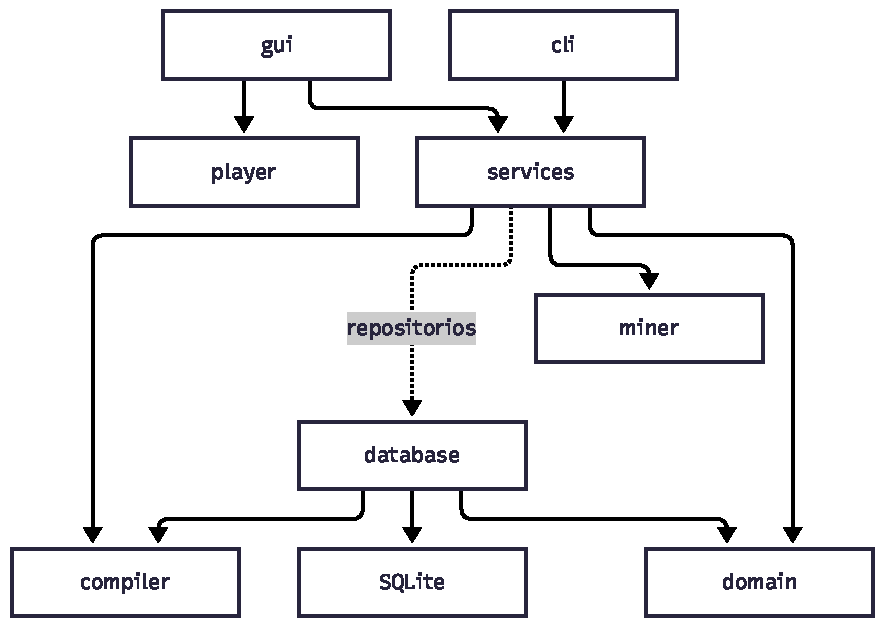
\includegraphics[width=0.6\textwidth]{figures/architecture.pdf}
	\caption{Diagrama de Arquitectura}
\end{figure}


La separación en bibliotecas busca reducir el acoplamiento entre componentes y delimitar sus
responsabilidades. La interfaz gráfica y la interfaz de línea de comandos comparten una capa de
servicios que expone las operaciones de la aplicación y coordina los subsistemas necesarios.
Esto permite reutilizar la lógica de la aplicación y realizar cambios internos de manera más
sencilla.

\subsection{Base de Datos}

\subsubsection*{Modelo Relacional}

\subsubsection*{Modelos de Dominio}

\subsubsection*{Repositorios}

\subsubsection*{Conexión}

\subsection{Minero}

La biblioteca utilizada para la extracción de metadatos es \textbf{TagLib}, principalmente porque ofrece
una facilidad para ampliar el sistema a otros formatos de audio. A pesar de la existencia de bibliotecas
más ligeras y enfocadas puramente en las etiquetas \texttt{ID3v2.4}, mi principal objetivo a futuro
con \textbf{8-Track} es el soporte de archivos \textbf{Hi-Res}.

\subsubsection*{Extracción de Metadatos}

La extracción de metadatos ocurre de manera recursiva buscando archivos cuya extensión
de formato sea exactamente \texttt{.mp3}. Para cada archivo se extraen título, artista, álbum,
género, año y número de pista. Para etiquetas faltantes, se utilizan los siguientes \texttt{fallbacks}:

\begin{itemize}
	\item \textbf{Texto}: \enquote{Unknown}
	\item \textbf{Año}: 2026
	\item \textbf{Número de Pista}: 1
\end{itemize}

Para desacoplar el minero de la base de datos y mantener la simplicidad en las pruebas unitarias,
el método principal \texttt{mine} recibe como argumento una función \textit{callback}. De este modo,
el minero permanece aislado y el comportamiento asociado a cada resultado se define externamente:
por ejemplo, imprimir los metadatos, acumularlos en memoria o guardarlos directamente en la base
de datos.

Por simplicidad, el reescaneo vuelve a leer los metadatos de todos los archivos
\texttt{.mp3} del directorio, aunque ya estén registrados en la biblioteca, y no
notifica a la base de datos sobre los archivos que fueron eliminados. Además,
si no es posible extraer los metadatos de un archivo, este simplemente se ignora.

\begin{figure}[htbp]
	\centering
	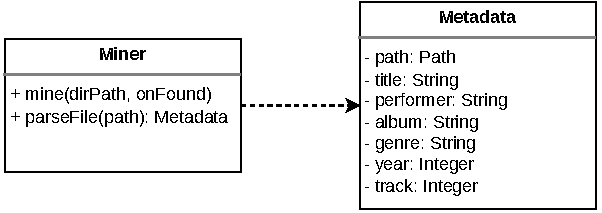
\includegraphics[width=0.6\textwidth]{figures/miner.pdf}
	\caption{Diagrama UML del minero}
\end{figure}

\subsubsection*{Extracción de Carátulas}

La extracción de carátulas se realiza mediante un segundo minero, \texttt{CoverMiner}. Este se
encarga de extraer los \textit{frames} \texttt{APIC} incrustados en los archivos \texttt{.mp3}
de la biblioteca, identificar cuáles corresponden al \textbf{artista} y al \textbf{álbum},
y guardarlas en disco.

\begin{figure}[H]
	\centering
	\begin{minipage}[t]{0.25\textwidth}
		\centering
		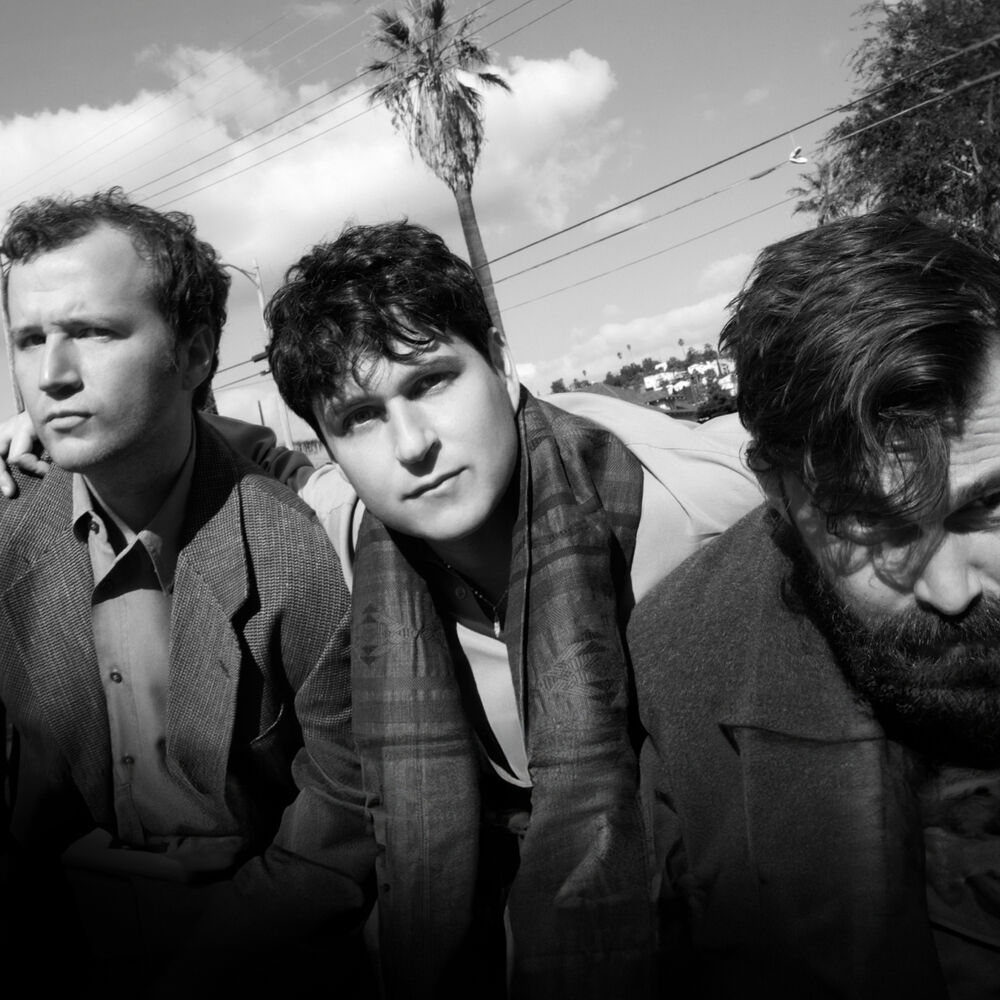
\includegraphics[width=\linewidth]{screnshoots/vampire.jpg}
		\par\smallskip
		\textbf{Artista}
	\end{minipage}%
	\hspace{0.04\textwidth}%
	\begin{minipage}[t]{0.25\textwidth}
		\centering
		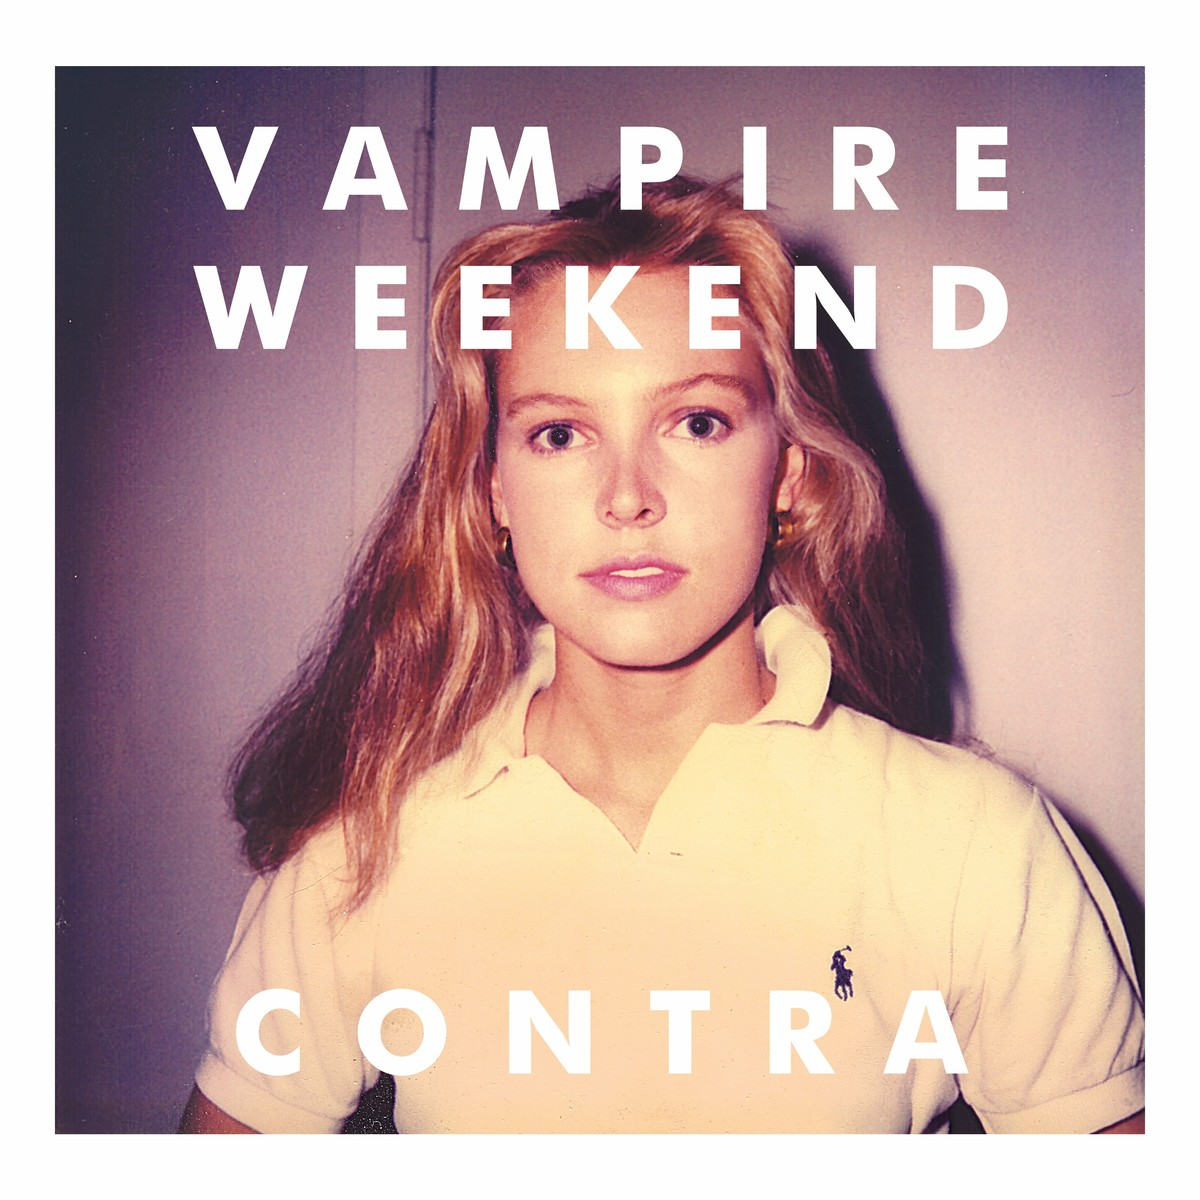
\includegraphics[width=\linewidth,trim=66bp 66bp 66bp 66bp,clip]{screnshoots/contra.jpg}
		\par\smallskip
		\textbf{Álbum}
	\end{minipage}
	\caption{Carátulas de artista y álbum}
\end{figure}

Primero, el minero comprueba si la imagen ya existe en la caché. Si no se encuentra, busca un
\textit{frame} \texttt{APIC} dentro del archivo \texttt{.mp3} y selecciona la imagen de mayor
jerarquía, con el siguiente orden de prioridad:

\begin{itemize}
	\item \textbf{Álbum}: \texttt{FrontCover} $\rightarrow$ \texttt{Other}
	\item \textbf{Artista}: \texttt{Artist} $\rightarrow$ \texttt{LeadArtist} $\rightarrow$ \texttt{Band}
\end{itemize}

Si no existe ninguna imagen, el escaneo continúa y no se guarda nada en la caché. Para evitar
búsquedas repetidas, el minero recuerda durante el escaneo los artistas y álbumes que ya intentó resolver sin éxito.

\subsubsection*{Caché de Carátulas}

Las imágenes extraídas se almacenan en el directorio \texttt{covers}, dentro de la ubicación de datos
de la aplicación.

Cada imágen se identifica con una clave sobre la cual se aplica una función hash \textbf{SHA-256}, cuya representación
hexadecimal se utiliza como nombre del archivo.

\begin{table}[htbp]
	\centering
	\begin{tabular}{ll}
		\hline
		\textbf{Tipo} & \textbf{Clave}                                   \\
		\hline
		Álbum         & \texttt{<ruta de la carpeta>|<nombre del álbum>} \\
		Artista       & \texttt{<nombre del artista>}                    \\
		\hline
	\end{tabular}
	\caption{Construcción de la clave de cada imagen}
\end{table}

\texttt{CoverStore} permite recuperar la ruta de una imagen recalculando su \textit{hash}, ya sea a
partir de la ruta de la carpeta y el nombre del álbum, o a partir del nombre del artista.
La ruta se calcula incluso cuando el archivo no existe, por lo que verificar su existencia
le corresponde a quien la consulta.

\subsection{MuQL}

\subsubsection*{Gramática}

\subsubsection*{Compilador}

\subsection{Servicios}

\subsection{Reproductor}

\subsection{Interfaz Gráfica}

\subsection{Interfaz de Terminal}
